\section{Quantification of Global Sampling}
\label{sec:global}

%\textcolor{blue}{DWS comment: Please address questions in TeX file.}

With ideal trajectory data, one would hope to be able to compute arbitrary observables with reasonably small error bars.
During a simulation, it is not uncommon to monitor specific observables of interest, but after the data are obtained, it may prove necessary to compute observables not previously considered.
These points motivate the task of estimating global sampling quality, which can be framed most simply in the context of single-trajectory data:
``Among the very large number of simulation frames (snapshots), how many are statistically independent?''
This number is called the \emph{effective sample size.}
From a dynamical perspective evoking auto-correlation ideas, which also apply to Monte Carlo data, how long must one wait before the system completely loses memory of its prior configuration?
%\textcolor{red}{PNP comment: I left a question about this section in the corresponding issue thread.}
The methods noted in this section build on ideas already presented in Sec.\ \ref{sec:quick} on qualitative sampling analysis, but attempt to go a step further to quantify sampling quality.

We emphasize that \emph{no single method described here has emerged as a clear best practice.}
However, because the global assessment methods provide a powerful window into overall sampling quality, which could easily be masked in the analysis of single observables (Sec.\ \ref{sec:specific}), we strongly encourage their use.
The reader is encouraged to try one or more of the approaches in order to understand the limitations of their data.

%\textcolor{red}{PNP comment: I removed a full paragraph here because I think that as written, it pigeonholes biomolecular simulations as the only ones for which one can define reasonable distance metrics.  This is simply not true.  I suspect that the materials community hasn't thought as much about distance measures, but I've certainly used them (and am writing a paper where we reference it specifically).  I think this section needs to have a wider scope that embraces the possibility that materials scientists will use ideas like RMSD.}
%\subsection{Scope and a key caveat}
%\textcolor{red}{PNP comment; I left a question about this section in the corresponding issue thread.}
%The discussion here will focus largely on biomolecular systems, or more precisely, on systems for which it is straightforward to define a meaningful scalar distance between configurations, such as an RMSD which quantifies configurational similarity or an analogous quantity for the full phase-space.
%Recall that a configuration is full set of $x, y, z$ coordinates describing a system, and ``phase space'' refers to the full set of configurational and momentum coordinates.

A key caveat is needed before proceeding.
Analysis of trajectory data generally cannot make inferences about parts of configuration space not visited \cite{Grossfield2009}.
It is generally impossible to know whether configurational states absent from a trajectory are appropriately absent because they are highly improbable (extremely high energy) or because the simulation simply failed to visit them because of a high barrier or random chance.

\subsection{Global sampling assessment for a single trajectory}
Two methods applicable for a single trajectory were previously introduced by some of the present authors, exploiting the fact that trajectories typically are correlated in time.
That is, each configuration evolves from and is most similar to the immediately preceding configuration;
this picture holds for standard MD and Markov-chain MC.
Both analysis methods are implemented as part of the software package LOOS \cite{LOOS,LOOS-JCC}.

\begin{figure}
  \centering
  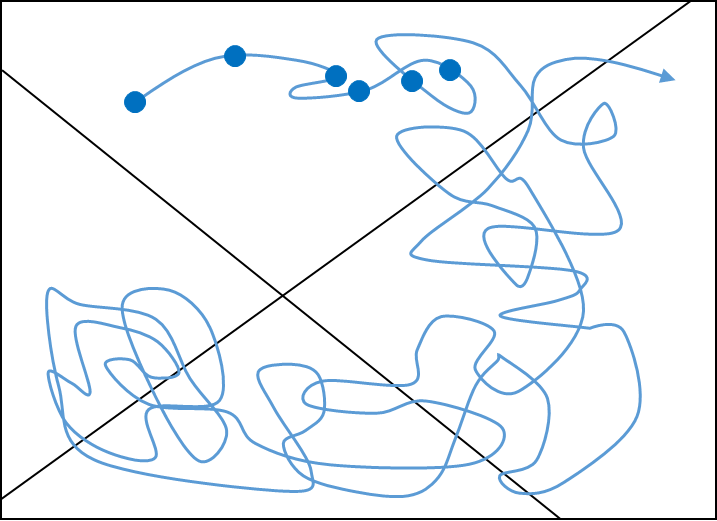
\includegraphics[width=0.8\linewidth]{decorr-graphic.png}
  \caption{The basis for ``decorrelation analysis'' \cite{Lyman2007a}.
  From a continuous trajectory (blue curve), configurations can be extracted at equally spaced time points (filled circles) with each such configuration categorized as belonging to one of a set of arbitrary states (delineated by straight black lines).  
  If the configurations are statistically independent -- if they are sufficiently decorrelated -- then their statistical behavior will match that predicted by a multinomial distribution consistent with the trajectory's fractional populations in each state.
  A range of time-spacings can be analyzed to determined if and when such independence occurs.}
  \label{fig:decorr}
\end{figure}

Lyman and Zuckerman proposed a global ``decorrelation'' analysis by mapping a trajectory to a discretization of configuration space (set of all $x, y, z$ coordinates) and analyzing the resulting statistics \cite{Lyman2007a}.
%\textcolor{red}{Would be helpful to clarify what this configuration space is.  Am I incorrect in assuming it is the full 6N-dimensional phase-space?  Other comments embedded in the .tex file as commented lines.}
Configuration space is discretized into bins based on Voronoi cells of structurally similar configurations,  e.g., using RMSD defined in Eq.\ \eqref{eq:rmsd} or another configurational similarity measure; reference configurations for the Voronoi binning are chosen at random or more systematically as described in \cite{Lyman2007a}.
%\textcolor{red}{Again, I have no idea what this means.  This problem could potentially be solved by definining the RMSD ideas a few sections up where they are first introduced.  Voronoi cells as I understand them define a set of ``nearest-neighbor'' domains, relative, e.g.\ to special points.  What are these special points, how are the Voronoi cells drawn?  Can this be stated more intuitively?}
Once configuration space is discretized, the trajectory frames can be classified accordingly, leading to a discrete (i.e., 'multinomial') distribution (Fig.\ \ref{fig:decorr}).
The analysis method is based on the observation that the variance for any bin of a multinomial distribution is known, given the bin populations (from trajectory counts) and a specified number of independent samples drawn from the distribution \cite{Lyman2007a}.
%\textcolor{red}{Is reference to the multinomial distribution necessary?  I find myself distracted by that word, wanting to know why that appears in the discretized phase-space, and why it's relevant for MD.}
The knowledge of the expected variance allows testing of increasing waiting times between configurations drawn from the trajectory to determine when and if the variance approaches that expected for independent samples.
The minimum waiting time yielding agreement with ideal (i.e., uncorrelated) statistics yields an estimate for the decorrelation/memory time, which in turns implies an overall effective sample size. 
%\textcolor{red}{Is this really about decorrelation times?  Perhaps I'm understanding wrong, but it seems like you're trying to address the problem of testing that all of phase-space has been sampled multiple times.}



A second method, employing block covariance analysis (BCOM), was presented by Romo and Grossfield \cite{Romo2011} building on ideas by Hess \cite{Hess2002}.  In essence, the method combines two standard error analysis techniques --- block averaging \cite{Flyvbjerg-1989} and bootstrapping \cite{Tibshirani1998} --- with covariance overlap, which quantitatively measures the similarity of modes determined from principal component analysis (PCA)\cite{Hess2002}.  PCA in essence generates a new coordinate system for representing the fluctuation in the system while tracking the importance of each vector; the central idea of the method is to exploit the fact that as sampling improves, the modes generated by PCA should become more similar, and the covariance overlap will approach unity in the limit of infinite sampling.

When applying BCOM, the principal components are computed from subsets of the trajectory, and the similarity of the modes evaluated as a function of subset size; as the subsets get larger, the resulting modes become more similar.  This is done both for contiguous blocks of trajectory data (block averaging), and again for randomly chosen subsets of trajectory frames (bootstrapping); taking the ratio of the two values as a function of block size yields the degree of correlation in the data.  Fitting that ratio to a sum of exponentials allows one to extract the relaxation times in the sampling.  The key advantage of this method over others is that it implicitly takes into account the number of substates; the longest correlation time is the time required not to make a transition, but to sample a scattering of the relevant states. 

\subsection{Global sampling assessment for multiple independent trajectories}
\label{sec:globalMultiTraj}
When sampling is performed using multiple independent trajectories (whether MD or MC), additional care is required.
Analyses based solely on the assumption of sequential correlations may break down because of the unknown relationship between separate trajectories.

Zhang et al.\ extended the decorrelation/variance analysis noted above, while still retaining the basic strategy of inferring sample size based on variance \cite{Zhang2010}.
To enable assessment of multiple trajectories, the new approach focused on conformational state populations, arguing that the states fundamentally underlie equilibrium observables.
Here, a state is defined as a finite region of configuration space, which ideally consists of configurations among which transitions are faster than transitions among states; 
in practice, such states can be approximated based on kinetic-clustering Voronoi cells according to the inter-state transition times \cite{Zhang2010}.
%\textcolor{red}{How is the word ``states'' being used in this sentence?  Are these microstates, i.e.\ phase-space points?  What does it mean to say states underlie equilibrium observables?  The latter can be computed as averages over (micro?)states?}
Once states are defined, the approach then uses the variances in state populations among trajectories to estimate the effective sample size, motivated by the decorrelation approach \cite{Lyman2007a} described above.
%\textcolor{red}{What is the effective sample size?  Number of independent trajectory frames?}

Nemec and Hoffmann proposed related sampling measures geared specifically for analyzing and comparing multiple trajectories \cite{Nemec2017}.
These measures again do not require user input of specific observables but only a measure of the difference between conformations, which was taken to the be the RMSD.
Nemec and Hoffmann provide formulas for quantifying the conformational overlap among trajectories (addressing whether the same configurational states were sampled) and the density agreement (addressing whether conformational regions were  sampled with equal probabilities).


